\fichetrue
\proftrue
\tdfalse
\coursfalse



\def\xxnumchapitre{Révisions 3 \vspace{.2cm}}
\def\xxchapitre{\hspace{.12cm} Modélisation par fonction de transfert et schéma-blocs}

\def\xxposongletx{2}
\def\xxposonglettext{1.45}
\def\xxposonglety{19}%16

\def\xxonglet{Cy 01 -- Rév 3}

\def\xxactivite{Fiche}


\def\xxpied{%
Cycle 01 -- Modéliser le comportement des systèmes multiphysiques\\
Révision 3 -- \xxactivite%
}

\setcounter{secnumdepth}{5}
%---------------------------------------------------------------------------

\iflivret
\pagestyle{empty}


%%%%%%%% PAGE DE GARDE COURS
\ifcours
% ==== BANDEAU DES TITRES ==== 
\begin{tikzpicture}[remember picture,overlay]
\node at (current page.north west)
{\begin{tikzpicture}[remember picture,overlay]
\node[anchor=north west,inner sep=0pt] at (0,0) {\includegraphics[width=\paperwidth]{\thechapterimage}};
\draw[anchor=west] (-2cm,-8cm) node [line width=2pt,rounded corners=15pt,draw=ocre,fill=white,fill opacity=0.6,inner sep=40pt]{\strut\makebox[22cm]{}};
\draw[anchor=west] (1cm,-8cm) node {\huge\sffamily\bfseries\color{black} %
\begin{minipage}{1cm}
\rotatebox{90}{\LARGE\sffamily\textsc{\color{ocre}\textbf{\xxnumpartie}}}
\end{minipage} \hfill
\begin{minipage}[c]{14cm}
\begin{titrepartie}
\begin{flushright}
\renewcommand{\baselinestretch}{1.1} 
\Large\sffamily\textsc{\textbf{\xxpartie}}
\renewcommand{\baselinestretch}{1} 
\end{flushright}
\end{titrepartie}
\end{minipage} \hfill
\begin{minipage}[c]{3.5cm}
{\large\sffamily\textsc{\textbf{\color{ocre} \discipline}}}
\end{minipage} 
 };
\end{tikzpicture}};
\end{tikzpicture}
% ==== FIN BANDEAU DES TITRES ==== 


% ==== ONGLET 
\begin{tikzpicture}[overlay]
\node[shape=rectangle, 
      rounded corners = .25 cm,
	  draw= ocre,
	  line width=2pt, 
	  fill = ocre!10,
	  minimum width  = 2.5cm,
	  minimum height = 3cm,] at (18.3cm,0) {};
\node at (17.7cm,0) {\rotatebox{90}{\textbf{\Large\color{ocre}{\classe}}}};
%{};
\end{tikzpicture}
% ==== FIN ONGLET 


\vspace{3.5cm}

\begin{tikzpicture}[remember picture,overlay]
\draw[anchor=west] (-2cm,-6cm) node {\huge\sffamily\bfseries\color{black} %
\begin{minipage}{2cm}
\begin{center}
\LARGE\sffamily\textsc{\color{ocre}\textbf{\xxactivite}}
\end{center}
\end{minipage} \hfill
\begin{minipage}[c]{15cm}
\begin{titrechapitre}
\renewcommand{\baselinestretch}{1.1} 
\Large\sffamily\textsc{\textbf{\xxnumchapitre}}

\Large\sffamily\textsc{\textbf{\xxchapitre}}
\vspace{.5cm}

\renewcommand{\baselinestretch}{1} 
\normalsize\normalfont
\xxcompetences
\end{titrechapitre}
\end{minipage}  };
\end{tikzpicture}
\vfill

\begin{flushright}
\begin{minipage}[c]{.3\linewidth}
\begin{center}
\xxfigures
\end{center}
\end{minipage}\hfill
\begin{minipage}[c]{.6\linewidth}
\startcontents
%\printcontents{}{1}{}
\printcontents{}{1}{}
\end{minipage}
\end{flushright}

\begin{tikzpicture}[remember picture,overlay]
\draw[anchor=west] (4.5cm,-.7cm) node {
\begin{minipage}[c]{.2\linewidth}
\begin{flushright}

\includegraphics[width=2cm]{logoCC}
\end{flushright}
\end{minipage}
\begin{minipage}[c]{.2\linewidth}
\textsl{\xxauteur} \\
\textsl{\classe}
\end{minipage}
 };
\end{tikzpicture}

\newpage
\pagestyle{fancy}

%\newpage
%\pagestyle{fancy}

\else
\fi
%% FIN PAGE DE GARDE DES COURS

%%%%%%%% PAGE DE GARDE TD
\iftd

% BANDEAU EXO
\iflivret % SI LIVRET
\begin{tikzpicture}[remember picture,overlay]
\draw[anchor=west] (-2cm,-3.3cm) node {\huge\sffamily\bfseries\color{black} %
\begin{minipage}{5cm}
\begin{center}
\LARGE\sffamily\color{ocre}\textbf{\textsc{\xxactivite}}

\begin{center}
\xxfigures
\end{center}

\end{center}
\end{minipage} \hfill
\begin{minipage}[c]{12cm}
\begin{titrechapitre}
\renewcommand{\baselinestretch}{1.1} 
\large\sffamily\textbf{\textsc{\xxtitreexo}}

\small\sffamily{\textbf{\textit{\color{black!70}\xxsourceexo}}}
\vspace{.5cm}

\renewcommand{\baselinestretch}{1} 
\normalsize\normalfont
\xxcompetences
\end{titrechapitre}
\end{minipage}};
\end{tikzpicture}
\else % ELSE NOT LIVRET
\begin{tikzpicture}[remember picture,overlay]
\draw[anchor=west] (-2cm,-4.5cm) node {\huge\sffamily\bfseries\color{black} %
\begin{minipage}{5cm}
\begin{center}
\LARGE\sffamily\color{ocre}\textbf{\textsc{\xxactivite}}

\begin{center}
\xxfigures
\end{center}

\end{center}
\end{minipage} \hfill
\begin{minipage}[c]{12cm}
\begin{titrechapitre}
\renewcommand{\baselinestretch}{1.1} 
\large\sffamily\textbf{\textsc{\xxtitreexo}}

\small\sffamily{\textbf{\textit{\color{black!70}\xxsourceexo}}}
\vspace{.5cm}

\renewcommand{\baselinestretch}{1} 
\normalsize\normalfont
\xxcompetences
\end{titrechapitre}
\end{minipage}};
\end{tikzpicture}

\fi

\else   % FIN IF TD
\fi


%%%%%%%% PAGE DE GARDE FICHE
\iffiche
\begin{tikzpicture}[remember picture,overlay]
\node at (current page.north west)
{\begin{tikzpicture}[remember picture,overlay]
\draw[anchor=west] (-2cm,-2.25cm) node [line width=2pt,rounded corners=15pt,draw=ocre,fill=white,fill opacity=0.6,inner sep=40pt]{\strut\makebox[22cm]{}};
\draw[anchor=west] (1cm,-2.25cm) node {\huge\sffamily\bfseries\color{black} %
\begin{minipage}{1cm}
\rotatebox{90}{\LARGE\sffamily\textsc{\color{ocre}\textbf{\xxnumpartie}}}
\end{minipage} \hfill
\begin{minipage}[c]{14cm}
\begin{titrepartie}
\begin{flushright}
\renewcommand{\baselinestretch}{1.1} 
\large\sffamily\textsc{\textbf{\xxpartie} \\} 

\vspace{.2cm}

\normalsize\sffamily\textsc{\textbf{\xxnumchapitre -- \xxchapitre}}
\renewcommand{\baselinestretch}{1} 
\end{flushright}
\end{titrepartie}
\end{minipage} \hfill
\begin{minipage}[c]{3.5cm}
{\large\sffamily\textsc{\textbf{\color{ocre} \discipline}}}
\end{minipage} 
 };
\end{tikzpicture}};
\end{tikzpicture}

\iflivret % SI LIVRET
\begin{tikzpicture}[overlay]
\node[shape=rectangle, 
      rounded corners = .25 cm,
	  draw= ocre,
	  line width=2pt, 
	  fill = ocre!10,
	  minimum width  = 2.5cm,
	  minimum height = 2.5cm,] at (18.5cm,.5cm) {};
\node at (17.9cm,.5cm) {\rotatebox{90}{\textsf{\textbf{\large\color{ocre}{\classe}}}}};
%{};
\end{tikzpicture}
\else  % SI PAS LIVRET
\iftd %% SI TD et PAS LIVRET
\begin{tikzpicture}[overlay]
\node[shape=rectangle, 
      rounded corners = .25 cm,
	  draw= ocre,
	  line width=2pt, 
	  fill = ocre!10,
	  minimum width  = 2.5cm,
	  minimum height = 2.5cm,] at (18.6cm,0.9cm) {};
\node at (18cm,0.9cm) {\rotatebox{90}{\textsf{\textbf{\large\color{ocre}{\classe}}}}};
%{};
\end{tikzpicture}

\else % FIN DU SI TD PAS LIVRET 
\begin{tikzpicture}[overlay]
\node[shape=rectangle, 
      rounded corners = .25 cm,
	  draw= ocre,
	  line width=2pt, 
	  fill = ocre!10,
	  minimum width  = 2.5cm,
%	  minimum height = 2.5cm,] at (18.5cm,1.1cm) {};
	  minimum height = 2.5cm,] at (18.6cm,0.5cm) {};
\node at (18cm,0.5cm) {\rotatebox{90}{\textsf{\textbf{\large\color{ocre}{\classe}}}}};
%{};
\end{tikzpicture}
\fi
\fi
\else
\fi



\else
\pagestyle{empty}


%%%%%%%% PAGE DE GARDE COURS
\ifcours
% ==== BANDEAU DES TITRES ==== 
\begin{tikzpicture}[remember picture,overlay]
\node at (current page.north west)
{\begin{tikzpicture}[remember picture,overlay]
\node[anchor=north west,inner sep=0pt] at (0,0) {\includegraphics[width=\paperwidth]{\thechapterimage}};
\draw[anchor=west] (-2cm,-8cm) node [line width=2pt,rounded corners=15pt,draw=ocre,fill=white,fill opacity=0.6,inner sep=40pt]{\strut\makebox[22cm]{}};
\draw[anchor=west] (1cm,-8cm) node {\huge\sffamily\bfseries\color{black} %
\begin{minipage}{1cm}
\rotatebox{90}{\LARGE\sffamily\textsc{\color{ocre}\textbf{\xxnumpartie}}}
\end{minipage} \hfill
\begin{minipage}[c]{14cm}
\begin{titrepartie}
\begin{flushright}
\renewcommand{\baselinestretch}{1.1} 
\Large\sffamily\textsc{\textbf{\xxpartie}}
\renewcommand{\baselinestretch}{1} 
\end{flushright}
\end{titrepartie}
\end{minipage} \hfill
\begin{minipage}[c]{3.5cm}
{\large\sffamily\textsc{\textbf{\color{ocre} \discipline}}}
\end{minipage} 
 };
\end{tikzpicture}};
\end{tikzpicture}
% ==== FIN BANDEAU DES TITRES ==== 


% ==== ONGLET 
\begin{tikzpicture}[overlay]
\node[shape=rectangle, 
      rounded corners = .25 cm,
	  draw= ocre,
	  line width=2pt, 
	  fill = ocre!10,
	  minimum width  = 2.5cm,
	  minimum height = 3cm,] at (18.3cm,0) {};
\node at (17.7cm,0) {\rotatebox{90}{\textbf{\Large\color{ocre}{\classe}}}};
%{};
\end{tikzpicture}
% ==== FIN ONGLET 


\vspace{3.5cm}

\begin{tikzpicture}[remember picture,overlay]
\draw[anchor=west] (-2cm,-6cm) node {\huge\sffamily\bfseries\color{black} %
\begin{minipage}{2cm}
\begin{center}
\LARGE\sffamily\textsc{\color{ocre}\textbf{\xxactivite}}
\end{center}
\end{minipage} \hfill
\begin{minipage}[c]{15cm}
\begin{titrechapitre}
\renewcommand{\baselinestretch}{1.1} 
\Large\sffamily\textsc{\textbf{\xxnumchapitre}}

\Large\sffamily\textsc{\textbf{\xxchapitre}}
\vspace{.5cm}

\renewcommand{\baselinestretch}{1} 
\normalsize\normalfont
\xxcompetences
\end{titrechapitre}
\end{minipage}  };
\end{tikzpicture}
\vfill

\begin{flushright}
\begin{minipage}[c]{.3\linewidth}
\begin{center}
\xxfigures
\end{center}
\end{minipage}\hfill
\begin{minipage}[c]{.6\linewidth}
\startcontents
%\printcontents{}{1}{}
\printcontents{}{1}{}
\end{minipage}
\end{flushright}

\begin{tikzpicture}[remember picture,overlay]
\draw[anchor=west] (4.5cm,-.7cm) node {
\begin{minipage}[c]{.2\linewidth}
\begin{flushright}

\includegraphics[width=2cm]{logoCC}
\end{flushright}
\end{minipage}
\begin{minipage}[c]{.2\linewidth}
\textsl{\xxauteur} \\
\textsl{\classe}
\end{minipage}
 };
\end{tikzpicture}

\newpage
\pagestyle{fancy}

%\newpage
%\pagestyle{fancy}

\else
\fi
%% FIN PAGE DE GARDE DES COURS

%%%%%%%% PAGE DE GARDE TD
\iftd

% BANDEAU EXO
\iflivret % SI LIVRET
\begin{tikzpicture}[remember picture,overlay]
\draw[anchor=west] (-2cm,-3.3cm) node {\huge\sffamily\bfseries\color{black} %
\begin{minipage}{5cm}
\begin{center}
\LARGE\sffamily\color{ocre}\textbf{\textsc{\xxactivite}}

\begin{center}
\xxfigures
\end{center}

\end{center}
\end{minipage} \hfill
\begin{minipage}[c]{12cm}
\begin{titrechapitre}
\renewcommand{\baselinestretch}{1.1} 
\large\sffamily\textbf{\textsc{\xxtitreexo}}

\small\sffamily{\textbf{\textit{\color{black!70}\xxsourceexo}}}
\vspace{.5cm}

\renewcommand{\baselinestretch}{1} 
\normalsize\normalfont
\xxcompetences
\end{titrechapitre}
\end{minipage}};
\end{tikzpicture}
\else % ELSE NOT LIVRET
\begin{tikzpicture}[remember picture,overlay]
\draw[anchor=west] (-2cm,-4.5cm) node {\huge\sffamily\bfseries\color{black} %
\begin{minipage}{5cm}
\begin{center}
\LARGE\sffamily\color{ocre}\textbf{\textsc{\xxactivite}}

\begin{center}
\xxfigures
\end{center}

\end{center}
\end{minipage} \hfill
\begin{minipage}[c]{12cm}
\begin{titrechapitre}
\renewcommand{\baselinestretch}{1.1} 
\large\sffamily\textbf{\textsc{\xxtitreexo}}

\small\sffamily{\textbf{\textit{\color{black!70}\xxsourceexo}}}
\vspace{.5cm}

\renewcommand{\baselinestretch}{1} 
\normalsize\normalfont
\xxcompetences
\end{titrechapitre}
\end{minipage}};
\end{tikzpicture}

\fi

\else   % FIN IF TD
\fi


%%%%%%%% PAGE DE GARDE FICHE
\iffiche
\begin{tikzpicture}[remember picture,overlay]
\node at (current page.north west)
{\begin{tikzpicture}[remember picture,overlay]
\draw[anchor=west] (-2cm,-2.25cm) node [line width=2pt,rounded corners=15pt,draw=ocre,fill=white,fill opacity=0.6,inner sep=40pt]{\strut\makebox[22cm]{}};
\draw[anchor=west] (1cm,-2.25cm) node {\huge\sffamily\bfseries\color{black} %
\begin{minipage}{1cm}
\rotatebox{90}{\LARGE\sffamily\textsc{\color{ocre}\textbf{\xxnumpartie}}}
\end{minipage} \hfill
\begin{minipage}[c]{14cm}
\begin{titrepartie}
\begin{flushright}
\renewcommand{\baselinestretch}{1.1} 
\large\sffamily\textsc{\textbf{\xxpartie} \\} 

\vspace{.2cm}

\normalsize\sffamily\textsc{\textbf{\xxnumchapitre -- \xxchapitre}}
\renewcommand{\baselinestretch}{1} 
\end{flushright}
\end{titrepartie}
\end{minipage} \hfill
\begin{minipage}[c]{3.5cm}
{\large\sffamily\textsc{\textbf{\color{ocre} \discipline}}}
\end{minipage} 
 };
\end{tikzpicture}};
\end{tikzpicture}

\iflivret % SI LIVRET
\begin{tikzpicture}[overlay]
\node[shape=rectangle, 
      rounded corners = .25 cm,
	  draw= ocre,
	  line width=2pt, 
	  fill = ocre!10,
	  minimum width  = 2.5cm,
	  minimum height = 2.5cm,] at (18.5cm,.5cm) {};
\node at (17.9cm,.5cm) {\rotatebox{90}{\textsf{\textbf{\large\color{ocre}{\classe}}}}};
%{};
\end{tikzpicture}
\else  % SI PAS LIVRET
\iftd %% SI TD et PAS LIVRET
\begin{tikzpicture}[overlay]
\node[shape=rectangle, 
      rounded corners = .25 cm,
	  draw= ocre,
	  line width=2pt, 
	  fill = ocre!10,
	  minimum width  = 2.5cm,
	  minimum height = 2.5cm,] at (18.6cm,0.9cm) {};
\node at (18cm,0.9cm) {\rotatebox{90}{\textsf{\textbf{\large\color{ocre}{\classe}}}}};
%{};
\end{tikzpicture}

\else % FIN DU SI TD PAS LIVRET 
\begin{tikzpicture}[overlay]
\node[shape=rectangle, 
      rounded corners = .25 cm,
	  draw= ocre,
	  line width=2pt, 
	  fill = ocre!10,
	  minimum width  = 2.5cm,
%	  minimum height = 2.5cm,] at (18.5cm,1.1cm) {};
	  minimum height = 2.5cm,] at (18.6cm,0.5cm) {};
\node at (18cm,0.5cm) {\rotatebox{90}{\textsf{\textbf{\large\color{ocre}{\classe}}}}};
%{};
\end{tikzpicture}
\fi
\fi
\else
\fi



\fi
\vspace{.5cm}
\pagestyle{fancy}
\thispagestyle{plain}
\setcounter{section}{0}


\section{Définitions}

%\begin{itemize}[label=\ding{112},font=\color{ocre}] 
%\item Une
%\item Une
%\end{itemize}

\begin{defi}[Fonction de transfert -- Transmittance] ~\\
Soit un système linéaire continu linéaire invariant dont on note le signal d'entrée $e$ et le signal de sortie $s$, régit par une équation différentielle à coefficient constants. Dans le domaine de Laplace et sous les conditions de Heaviside, on définit la fonction de transfert du système par la fonction $H$ telle que : 
$$
H(p)
=\dfrac{S(p)}{E(p)} 
= \dfrac{\sum\limits_{i=0}^{m} b_i p^i}{\sum\limits_{i=0}^{n} a_i p^i}
=\dfrac{N(p)}{D(p)}.
$$
 

\end{defi}

\begin{defi}[Classe, ordre, pôles et zéros] ~\\
$H(p)$ est une fonction rationnelle en $p$. En factorisant le numérateur et le
dénominateur, $H(p)$ peut s'écrire sous cette forme :
$$
H(p) = \dfrac{N(p)}{D(p)} =
K \dfrac{\left(p-z_1 \right)\left(p-z_2 \right)...\left(p-z_m \right)}{
p^{\alpha} \left(p-p_1 \right)\left(p-p_2 \right)...\left(p-p_n \right)}
$$


 \begin{itemize}
 \item Les $z_i$ sont les \textbf{zéros} de la fonction de transfert (réels ou
complexes).
\item Les $p_i$ sont les \textbf{pôles} de la fonction de transfert (réels ou
complexes).
\item \textbf{Le degré de $D(p)$ est appelé ordre $n$ du système ($n\geq m$ pour les
systèmes physiques).}
\item L'équation $D(p)=0$ est appelée équation caractéristique.
\item Le facteur constant $K$ est appelé gain du système.
\item S'il existe une (ou des) racines nulles d'ordre $\alpha$ de $D(p)$, un
terme $p^\alpha$ apparaît au dénominateur. \textbf{$\alpha$ est la classe (ou type) de
la fonction de transfert}. Il correspond au nombre d'intégrations pures du
système.
\end{itemize}


\end{defi}



\begin{defi}[Modélisation d'un bloc] ~\\

\noindent \begin{minipage}[c]{.75\linewidth}
Soit un système d'entrée $E(p)$, de sortie $S(p)$, caractérisé par une fonction
de transfert $H(p)$. Ce système est alors représenté par le schéma bloc ci-contre.
La relation entrée -- sortie du système se met alors sous la forme : 
$$
S(p) = E(p) \cdot H(p).
$$
\end{minipage} \hfill
\begin{minipage}[c]{.2\linewidth}
\begin{center}
\begin{tikzpicture}
\sbEntree{E}
\sbBloc{sys}{$\quad$H(p)$\quad$}{E} \sbRelier[$E(p)\quad$]{E}{sys}
\sbSortie{S}{sys} \sbRelier[$\quad S(p)$]{sys}{S}
\end{tikzpicture} 
\end{center}
\end{minipage}

\end{defi}

\begin{defi}[Modélisation d'un comparateur] ~\\
\noindent \begin{minipage}[c]{.65\linewidth}
Soit l'équation $S(p)=E_1(p)-E_2(p)$. Cette équation se traduit par le schéma ci-contre.
\end{minipage} \hfill
\begin{minipage}[c]{.3\linewidth}
\begin{center}

\begin{tikzpicture}
\sbEntree{E}
\sbComp{cp}{E}
\sbSortie[9]{S}{cp} 
\sbRelier[$E_1(p)$]{E}{cp}
\sbRelier[$S(p)=E_1(p)-E_2(p)$]{cp}{S}
\sbDecaleNoeudy[4]{S}{n}
\sbDecaleNoeudx[-14]{n}{n2}
\sbRelierxy[$E_2(p)$]{n2}{cp}
\end{tikzpicture} 
\end{center}
\end{minipage}


\end{defi}


\section{Algèbre de blocs}


\begin{warn}~\\
Pour modifier un schéma-blocs, il faut s'assurer que lorsque on modifie une partie du schéma, les grandeurs d'entrée et de sortie sont identiques avant et après la transformation.
\end{warn}

\begin{resultat}[Blocs en série] ~\\

\vspace{-.6cm}
\begin{center}
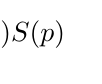
\begin{tikzpicture}
\sbEntree{E}
\sbBloc{sys}{$H_1(p) $}{E}
\sbRelier[$E(p)\quad $]{E}{sys}
\sbBloc{sys2}{$ H_2(p) $}{sys}
\sbRelier{sys}{sys2}
\sbSortie{S}{sys2} 
\sbRelier[$\quad S(p)$]{sys2}{S}

\begin{scope}[xshift=6.25cm]
\draw (0,0) node {$\Leftrightarrow$};
\end{scope}

\begin{scope}[xshift=7cm]
\sbEntree{E}
\sbBloc{sys}{$H_1(p) H_2(p) $}{E}
\sbRelier[$E(p)\quad $]{E}{sys}
\sbSortie{S}{sys} 
\sbRelier[$\quad S(p)$]{sys}{S}
\end{scope}
\end{tikzpicture} 

\end{center}

\end{resultat}


\begin{resultat}[Blocs en parallèle] ~\\

\vspace{-.6cm}

\begin{center}
\begin{tikzpicture}
\sbEntree{E}
\sbBloc{sys}{$H_1(p) $}{E}
\sbRelier[$E(p)\quad $]{E}{sys}
\sbSumb{cp}{sys}
\sbRelier{sys}{cp}

\sbDecaleNoeudy[4]{E}{n}
\sbBloc{sys2}{$H_2(p) $}{n}
\sbRelieryx{E-sys}{sys2}
\sbRelierxy{sys2}{cp}

\sbSortie{S}{cp} 
\sbRelier[$\quad S(p)$]{cp}{S}


\begin{scope}[xshift=4cm]
\draw (0,0) node {$\Leftrightarrow$};
\end{scope}

\begin{scope}[xshift=5cm]
\sbEntree{E}
\sbBloc{sys}{$H_1(p) +H_2(p) $}{E}
\sbRelier[$E(p)\quad $]{E}{sys}
\sbSortie{S}{sys} 
\sbRelier[$\quad S(p)$]{sys}{S}
\end{scope}
\end{tikzpicture} 
\end{center}

\end{resultat}


\begin{resultat}[Réduction de boucle -- À MAITRISER PARFAITEMENT] ~\\

\vspace{-.6cm}

\begin{center}
\begin{tikzpicture}
\sbEntree{E}
\sbComp{cp}{E}
\sbRelier[$E(p)\quad $]{E}{cp}
\sbBloc{sys}{$H_1(p) $}{cp}
\sbRelier{cp}{sys}
\sbSortie{S}{sys} 
\sbRelier[$\quad S(p)$]{sys}{S}

\sbDecaleNoeudy[4]{cp}{n}
\sbBloc{sys2}{$H_2(p) $}{n}
\sbRelierxy{sys2}{cp}
\sbRelieryx{sys-S}{sys2}
%
%\sbBloc{sys}{$H_1(p) $}{E}
%\sbRelier{E}{sys}
%
%\sbDecaleNoeudy[4]{E}{n}
%\sbBloc{sys2}{$H_2(p) $}{n}
%\sbRelieryx{E-sys}{sys2}
%\sbRelierxy{sys2}{cp}
%
%\sbSortie{S}{cp} 
%\sbRelier[$\quad S(p)$]{cp}{S}


\begin{scope}[xshift=5cm]
\draw (0,0) node {$\Leftrightarrow$};
\end{scope}

\begin{scope}[xshift=6cm]
\sbEntree{E}
\sbBloc{sys}{$\dfrac{H_1(p)}{1+H_1(p)H_2(p)} $}{E}
\sbRelier[$E(p)\quad $]{E}{sys}
\sbSortie{S}{sys} 
\sbRelier[$\quad S(p)$]{sys}{S}
\end{scope}
\end{tikzpicture} 
\end{center}

\end{resultat}


\begin{resultat}[Comparateurs en série] ~\\

\vspace{-.6cm}

\begin{center}
\begin{tikzpicture}
\sbEntree{E}
\sbComp{cp1}{E}
\sbComph{cp2}{cp1}
\sbSortie{S}{cp2} 

\sbRelier[$E(p)\quad $]{E}{cp1}
\sbRelier{cp1}{cp2}
\sbRelier[$\quad S(p)$]{cp2}{S}

\sbDecaleNoeudy[4]{E}{n1}
\sbDecaleNoeudy[-4]{E}{n2}
\sbRelierxy[$E_1(p)$]{n1}{cp1}
\sbRelierxy[$E_2(p)$]{n2}{cp2}


\begin{scope}[xshift=5cm]
\draw (0,0) node {$\Leftrightarrow$};
\end{scope}

\begin{scope}[xshift=6cm]
\sbEntree{E}
\sbComph{cp1}{E}
\sbComp{cp2}{cp1}
\sbSortie{S}{cp2} 

\sbRelier[$E(p)\quad $]{E}{cp1}
\sbRelier{cp1}{cp2}
\sbRelier[$\quad S(p)$]{cp2}{S}

\sbDecaleNoeudy[4]{E}{n1}
\sbDecaleNoeudy[-4]{E}{n2}
\sbRelierxy[$E_1(p)$]{n1}{cp2}
\sbRelierxy[$E_2(p)$]{n2}{cp1}
\end{scope}

\end{tikzpicture}
\end{center}
\end{resultat}


\begin{resultat}[Point de prélèvement] ~\\

\vspace{-.6cm}

\begin{center}
\begin{tikzpicture}
\sbEntree{E}
\sbBloc{b1}{$H_1(p) $}{E}
\sbSortie{S}{b1} 

\sbRelier[$E(p)\quad $]{E}{b1}
\sbRelier[$\quad S(p)$]{b1}{S}

\sbDecaleNoeudy[4]{S}{n1}
\sbBlocr{b2}{$H_2(p)$}{n1}
\sbRelieryx{b1-S}{b2}
\sbDecaleNoeudx[-4]{b2}{n2}
\sbRelier[$\quad R(p)\quad \quad $]{b2}{n2}

\begin{scope}[xshift=4cm]
\draw (0,0) node {$\Leftrightarrow$};
\end{scope}

\begin{scope}[xshift=8cm]
\sbEntree{E}
\sbBloc{b1}{$H_1(p)$}{E}
\sbSortie{S}{b1} 

\sbRelier[$E(p)\quad $]{E}{b1}
\sbRelier[$\quad S(p)$]{b1}{S}

\sbDecaleNoeudy[4]{E}{n1}
\sbDecaleNoeudx[2]{n1}{n2}
\sbBlocr{b2}{$H_2(p) H_1(p)$}{n2}
\sbRelieryx{E-b1}{b2}
\sbDecaleNoeudx[-6]{b2}{n3}
\sbRelier[$\quad R(p)\quad \quad $]{b2}{n3}
\end{scope}

\end{tikzpicture}
\end{center}

\end{resultat}



\section{Fonctions usuelles}



\begin{defi}[Fonction de transfert en boucle fermée -- FTBF] ~\\
\textit{Formule de Black}
\vspace{-.6cm}

\begin{minipage}[c]{.48\linewidth}
$$H(p)=\dfrac{S(p)}{E(p)}=\dfrac{H_1(p)}{1+H_1(p)H_2(p)}$$
\end{minipage}\hfill
\begin{minipage}[c]{.48\linewidth}
\begin{center}
\begin{tikzpicture}
\sbEntree{E}
\sbComp{cp}{E}
\sbRelier[$E(p)\quad $]{E}{cp}
\sbBloc[4]{sys}{$H_1(p) $}{cp}
\sbRelier[$\varepsilon(p)$]{cp}{sys}
\sbSortie[4]{S}{sys} 
\sbRelier[$\quad S(p)$]{sys}{S}

\sbDecaleNoeudy[4]{cp}{n}
\sbDecaleNoeudx[2]{n}{n2}
\sbBloc{sys2}{$H_2(p) $}{n2}
\sbRelierxy[$R(p)$]{sys2}{cp}
\sbRelieryx{sys-S}{sys2}
\end{tikzpicture}
\end{center} 
\end{minipage}
\end{defi}



\begin{defi}[Fonction de transfert en boucle ouverte -- FTBO] ~\\

\vspace{-.6cm}

\begin{minipage}[c]{.48\linewidth}
$$\text{FTBO}(p)=\dfrac{R(p)}{\varepsilon(p)}=H_1(p) H_2(p)$$
\end{minipage}\hfill
\begin{minipage}[c]{.48\linewidth}
\begin{center}
\begin{tikzpicture}
\sbEntree{E}
\sbComp{cp}{E}
\sbRelier[$E(p)\quad $]{E}{cp}
\sbBloc[4]{sys}{$H_1(p) $}{cp}
\sbRelier[$\varepsilon(p)$]{cp}{sys}
\sbSortie[4]{S}{sys} 
\sbRelier[$\quad S(p)$]{sys}{S}

\sbDecaleNoeudy[4]{cp}{n}
\sbDecaleNoeudx[2]{n}{n2}
\sbBloc{sys2}{$H_2(p) $}{n2}
\sbRelierxy[$R(p)$]{sys2}{cp}
\sbRelieryx{sys-S}{sys2}
\end{tikzpicture}
\end{center} 
\end{minipage}

\end{defi}

%
%\begin{defi}[Chaîne directe] ~\\
%
%\end{defi}
%
%
%
%\begin{defi}[L'écart] ~\\
%
%\end{defi}
%

\begin{defi}[Théorème de superposition] ~\\
Soit un système d'entrées $E_1$ et $E_2$ et de sortie $S$. On note $H_1=\dfrac{S}{E_1}$ lorsque $E_2$ est nulle et $H_2=\dfrac{S}{E_2}$ lorsque $E_1$ est nulle. En superposant, on a alors : $S=H_1 E_1 + H_2 E_2$.
\end{defi}



